\chapter{Construction works modelling}
\label{ch:constr:wm}

\section{Weirs}
\label{sec:weirs}
Weirs are considered as linear singularities.
Their use is possible in parallel computing (since release 6.2).
The number of weirs is specified by the keyword \telkey{NUMBER OF WEIRS}
(default value 0).
Information about weirs is given in the \telkey{WEIRS DATA FILE}.

A weir must be prepared in the mesh and consists of two boundary lines which are
actually linked by the weir.
In principle, these boundaries should be sufficiently far apart,
upstream and downstream of the weir.
The upstream and downstream boundary points should correspond 1 to 1,
and the distance between two points should be the same on both sides.
The following file gives an example of two weirs (the comments are part of the
file):
\begin{lstlisting}[language=bash]
Nb of weirs     Option for tangential velocity
      2                    0
---------------------------- singularity 1
Nb of points for 1 side
11
Points side 1
71 72 73 74 75 76 77 78 79 80 41
Points side 2
21 20 19 18 17 16 15 14 13 12 11
Level of the dyke
1.8 1.8 1.8 1.8 1.8 1.8 1.8 1.8 1.8 1.8 1.8
Flowrate coefficients
 .4  .4  .4  .4  .4  .4  .4  .4  .4  .4  .4
---------------------------- singularity 2
Nb of points
11
Points side 1
111 112 113 114 115 116 117 118 119 120 81
Points side 2
61 60 59 58 57 56 55 54 53 52 51
Level of the dyke
1.6 1.6 1.6 1.6 1.6 1.6 1.6 1.6 1.6 1.6 1.6
Flowrate coefficient
 .4  .4  .4  .4  .4  .4  .4  .4  .4  .4  .4
\end{lstlisting}

Line 2 indicates the number of weirs and then an option for the treatment
of tangential velocities on the weir, with the following meaning:

\begin{itemize}
\item 0: the velocities are null (recommended option),

\item 1: the velocities will be calculated with the Ch\'{e}zy
formula (as a function of the local free surface slope).
\end{itemize}

For each weir, it is then necessary to indicate:
the number of points for the first side of the weir (line 5 for the first weir)
and the list of their global numbers (line 7 for the first weir).
Note, that before and for release 6.1, the numbering to provide was not the
global one but the local numbering of the boundary defined in the
\telkey{BOUNDARY CONDITIONS FILE}.
However, it is necessary to provide the weirs number in the order of the
boundary points.

The numbers of their twin points on side 2 should be given on line 9 in the
reverse order.
On line 11, the level of the weir is specified for each couple of points
and at line 13 the discharge coefficient noted m.
All these data are repeated for all weirs.

The formulae used to calculate the discharge for each point are the following:

\begin{itemize}
\item unsubmerged weir: $Q=\mu \sqrt{2g}\ {\left(upstream-weir\right)}^{\frac{3}{2}}$,

\item submerged weir:
\[Q=\ {\left(\frac{2}{3}\sqrt{\frac{1}{3}}\right)}^{-1}\mu \sqrt{2g}
\left(downstream-weir\right)\sqrt{\left(upstream-weir\right)},\]

\item the weir is not submerged if:
\[upstream\ level<\frac{weir\ level+2 \times upstream\ level}{3}.\]
\end{itemize}
Depending on the shape and roughness of the weir, the value of $\mu$
is between 0.4 and 0.5.
However, the above formulae neglect the velocity of the upstream head in the
computation.
If this is not the case, the value of $\mu$ may be higher.

If the user wants to modify the different laws, it is possible to modify the
appropriate subroutines (\telfile{LOIDEN} and \telfile{LOINOY}).\\

The keyword \telkey{TYPE OF WEIRS} gives the method to treat weirs.
2 options are available:
\begin{itemize}
\item horizontal with same number of nodes upstream/downstream
(Historical solution with the \telfile{BORD} subroutine,
which is the default value),
\item general (new solution with sources points).
\end{itemize}


\section{Culverts}
\label{sec:culverts}
As for weirs, the keyword \telkey{NUMBER OF CULVERTS} (default value = 0)
specifies the number of culverts to be treated.
Culverts are described as couples of points between which flow may occur,
as a function of the respective water level at these points.
Since release 6.2 of \telemac{2D}, it is no longer necessary to describe
each culvert inflow and outflow as a source point.

There are two options to treat culverts in \telemac{2D}.
The choice can be done with \telkey{OPTION FOR CULVERTS}
(default value = 1).
For more information about this choice, the reader is invited to refer to the
\telemac{3D} theory guide.\\

Information about culvert characteristics is stored in the
\telkey{CULVERTS DATA FILE}.

The following file gives an example of a culvert:
\begin{lstlisting}[language=bash]
Relaxation, Number of culverts
0.2 1
I1  I2  CE1 CE2 CS1 CS2 LRG  HAUT1 CLP LBUS Z1  Z2  CV  C56 CV5 C5  CT  HAUT2 FRIC LENGTH CIRC D1  D2 A1 A2  AA
199 640 0.5 0.5 10  1.0 2.52 2.52  0   0.2  0.3 0.1 0.0 0.0 0.0 0.0 0.0 2.52  0.0  0.0    1    90. 0. 0. 90. 0

\end{lstlisting}

The relaxation coefficient is initially used to prescribe the discharge
in the culvert on a progressive basis in order to avoid the formation of an eddy.
Relaxation, at time $T$, between result computed at time $T$ and result
computed at previous time step.
A relaxation coefficient of 0.2 means that 20\% of time $T$ result is mixed
with 80\% of the previous result.
I1 and I2 are the numbers of each end of the culvert in the global point
numbering system.

The culvert discharge is calculated based on the formulae given
in the \telemac{3D} theory guide and in the release notes of \telemac{2D}:
CE1 and CE2 are the head loss coefficients of 1 and 2 when they are operating as
inlets.
CS1 and CS2 are the head loss coefficients of 1 and 2 when they are operating as
outlets.
LRG is the width of the culvert.
HAUT1 and HAUT2 are the heights of the construction work (in meters)
at the inlet and outlet.
The flow direction is also imposed through the keyword CLP:\\
CLP = 0, flow is allowed in both directions,\\
CLP = 1, flow is only allowed from section 1 to section 2,\\
CLP = 2, flow is only allowed from section 2 to section 1,\\
CLP = 3, no flow allowed.\\
LBUS is the linear head loss in the culvert, generally equal to
$\lambda {\kern 1pt} {\kern 1pt} {\kern 1pt} {\kern 1pt} {\kern 1pt} \frac{L}{D} $
where $L$ is the length of the pipe, $D$ its diameter and $l$ the friction
coefficient.
Z1 and Z2 are the levels of the inlet and outlet.
CV refers to the loss coefficient due to the presence of a valve and
C56 is the constant used to differentiate flow types 5 and 6 in the formulation
by Bodhaine.
C5 and CV5 represent correction coefficients to C1 and to CV coefficients
due to the occurrence of the type 5 flow in the Bodhaine formulation.
CT is the loss coefficient due to the presence of trash screens.
FRIC is the Manning Strikler coefficient.
LENGTH is the length of the culvert, and the culvert's shape can be specified
through the parameter CIRC (equal to 1 in
case of a circular section, 0 for a rectangular section).
A1 and A2 are the angles with respect to the $x$ axis.
D1 and D2 are the angles that the pipe makes with respect to the bottom,
in degrees.
For a vertical intake, the angle with the bottom will therefore be 90$^\circ$.
They are used to account for the current direction at source or sink point.
AA is a parameter which allows the user to choose whether A1 and A2 are
automatically computed by \telemac{2D}
or whether the data file values are used to set these angles:
AA=1 -- automatic angle; AA=0 -- user-set angle.


\section{Dykes breaches}
\label{sec:dykes}
\subsection{General overview}
\telemac{2D} allows simulating dykes breaching by suddenly or gradually
lowering the altitude of some points.
This feature is enabled using the logical keyword \telkey{BREACH} (default = NO).
The different kinds of breach developments are completely controlled by user
via the \telkey{BREACHES DATA FILE}.
Regardless the kind of breach development, to model this phenomenon,
it is necessary to know:
\begin{itemize}
\item the final width of the breach (the width is the longitudinal dimension
with respect to the channel flow direction),
\item the duration of the breaching process,
\item the final altitude of the breach.
\end{itemize}
Indeed the breach is represented in \telemac{2D} by a polygon (defined by users
in the \telkey{BREACHES DATA FILE}) within the altitude of mesh nodes lowers
with time according to the selected breach law.

Current state-of-the-art on the breaching of earthen dykes due to overtopping
flows shows that the dyke breaching expansion is progressive (non-instantaneous)
(\cite{Morris2009a,Risher2016,Wu2017,Rifai2017,Rifai2018,Rifai2019}, among
others), following two main phases (referred to as breach formation
and development period, respectively):
\begin{itemize}
\item Phase 1 - Deepening and lateral widening: as the overtopping flow depth and
velocity over the dyke increase, both breach deepening and widening are promoted
with a shift of the breach centerline toward the channel downstream end.
The breach sides collapse gradually. The breach expansion during this phase is
fast,
\item Phase 2 - Lateral widening: the main channel free surface decreases and the
flow depth starts stabilizing at its minimum level (approaching the main channel
critical flow depth). The breach development becomes slower, the upstream part of
the breach stops evolving, and deepening becomes moderate tending to stabilize.
The breach widens along the channel flow direction due to side slope failures.
\end{itemize}
The breach deepening (vertical incision of the breach) is faster than breach
widening (\cite{Morris2009b,Wahl2017,Rifai2017,Rifai2018}). When the breach bottom
reaches the foundation of the dyke or a non-erodible layer, no further deepening
of the breach is possible and lateral widening is controlling the breach
expansion until its stabilisation (i.e. fully formed breach, final width is
reached and erosion is stopped).

Selected empirical laws have been implemented in \telemac{2D} for simulating
the time evolution of the breach expansion (widening and deepening). They are
described here below. \\
As the flood period and inundation of the floodplain along with the dyke material
characteristics impose certain limits on breach growth, the empirical laws are
applied over a given duration.
The breach expansion continues until the breach
has expanded to its approximate maximum dimensions.

\begin{WarningBlock}{Warning:}
Therefore the final
(i.e. ultimate, maximum) breach
dimensions (width and bottom elevation), the duration of the breaching expansion
(or duration of each phase), must be estimated outside
of the \tel software by the user.
\end{WarningBlock}

These parameters are indeed mandatory
in the
\telkey{BREACHES DATA FILE} which contains the description and the
characteristics of
the breaching process; it will be described here below.
Except for the Froehlich model, the breach longitudinal shape is assumed
rectangular.

In addition to the breach expansion computation, it is important to define a
criterion to start
the breaching process. In the current release, 5 types of criteria are
available:

\begin{enumerate}
\item at a given time. This option can be chosen filling the
\telkey{BREACHES DATA FILE} with:
\begin{lstlisting}[language=bash]
# Option for breaching initiation
1
\end{lstlisting}

\item when the water level above the dyke
(the averaged value of water depth is computed for all points inside the
polygon defining the dyke) reaches a given value.
This option can be chosen filling the \telkey{BREACHES DATA FILE} with:
\begin{lstlisting}[language=bash]
# Option for breaching initiation
2
\end{lstlisting}

\item when the water level at a given point reaches a certain value.
This option can be chosen filling the \telkey{BREACHES DATA FILE} with:
\begin{lstlisting}[language=bash]
# Option for breaching initiation
3
\end{lstlisting}

\item when the water level at a given point reaches a certain value and when
the energy balance ($\Delta E$) defined as the difference between the upstream
head (channel side, $E_{riv}$) and downstream head (floodplain side, $E_{pla}$)
reaches a threshold value (see Figure \ref{fig:crit4+5}).
According to the way used to compute the energy balance, two options can be chosen:
\begin{itemize}
 \item the hydraulic head is computed at points (mesh nodes) given by user (3
   points are expected, see below).
   This option can be chosen filling the \telkey{BREACHES DATA FILE} with:
   \begin{lstlisting}[language=bash]
   # Option for breaching initiation
   4
   \end{lstlisting}
 \item the hydraulic head is automatically computed by \telemac{2D} taking an
   averaged value of points which are located on the border of the polygon
   used to define the breach
   (it is assumed that the border should represent the foot of the dyke).
   This option can be chosen filling the \telkey{BREACHES DATA FILE} with:
   \begin{lstlisting}[language=bash]
   # Option for breaching initiation
   5
   \end{lstlisting}
\end{itemize}
\end{enumerate}
\begin{figure}
\centering
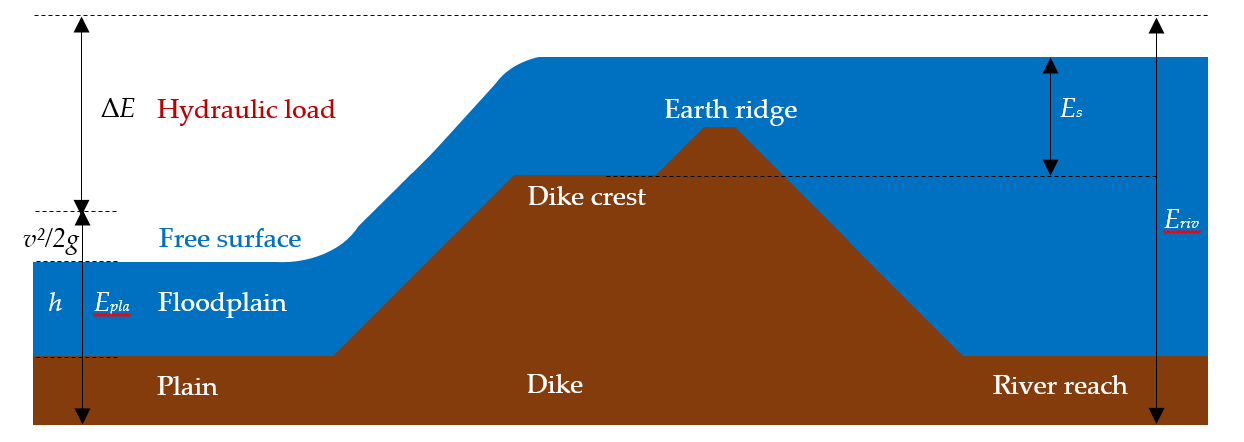
\includegraphics[width=\textwidth]{./graphics/goeury2022}
\caption{Scheme illustrating variables used to identify the initiation of breach
expansion on a profile across a levee (surmounted by an earth ridge). $v$ (m/s)
is the mean flow velocity \cite{Goeury2022}.}
\label{fig:crit4+5}
\end{figure}
Since release 7.0, it is possible to take into account a lateral growth
of the breach (dyke opening by widening and deepening).
Old breaching processes are not affected by this new feature: only the breach
deepening was taken into account in the breach computation.

Since release 8.3, several laws for lateral growth have been implemented and they
are described in the following section.

\subsection{Breach computation for rectangular shapes}
\subsubsection{Breach widening}
For the sake of simplicity, the following empirical laws are given assuming a
zero-value for the initial width of the breach.

\begin{itemize}
\item Linear widening \\
The time evolution breaching process is simulated with the following formula:
\begin{equation}
\begin{array}{lc}
B(t)=\dfrac{B_f}{T_f}t & \text{for}~t\leq T_f
\end{array}
\end{equation}
where $B_f$ is the final breach width, $T_f$ is the total duration of the breach
expansion in hours and $t$ in hours. \\
This law can be selected filling the \telkey{BREACHES DATA FILE} with:
\begin{lstlisting}[language=bash]
# Option for lateral growth
2
\end{lstlisting}

\item User-defined breach expansion formulations

The breach widening can be simulated according to a linear-time progression formula.
The user has the possibility to specify
one or two growth rates: to mimic the real breach widening the user can simulate
a breach that initially grows very quickly then slows down towards the end of
the development time. The formula is:
\begin{equation}
B(t)=\left\{
\begin{array}{lc}
E_{w1}t & \text{for}~t\leq T_1 \\
E_{w1}T_1+E_{w2}(t-T_1) & \text{for}~T_1\leq t \leq T_f
\end{array}
\right.
\end{equation}
with $t$ time in hours (after the initiation of breaching), $B$ = breach width
in meters, $T_1$ = duration of phase 1 in hours, $T_f$ = total duration of the
breach expansion (phase 1 and phase 2) in hours, $E_{w1}$ and $E_{w2}$ = breach
growth rates (m/h).
This law can be selected filling the \telkey{BREACHES DATA FILE} with:
\begin{lstlisting}[language=bash]
# Option for lateral growth
3
\end{lstlisting}
Information for defining these growth rate parameters could be obtained from
literature or physically-based models (\cite{FERC1988,Wahl1998,West2018}).
Using available datasets, Resio et al. (2009) concluded that the rate of breach
widening is ranging between 9 m/h for erosion-resistant soils (cohesive dykes)
and 60 m/h for erodible alluvial material (sand and gravel soils).
The widening rate can reach (rarely) 300 m/h for very erodible dykes.
USBR \cite{USBR1988} recommended a single breach widening rate of 91 m/h for
embankment dams - formula taking into account this rate is already implemented
for users who wish to apply it.
\item USBR formula (1988) \\
The breach widening is estimated as a function of time with the following linear
progression formula proposed by USBR \cite{USBR1988}:
\begin{equation}
\begin{array}{lc}
B(t)=91t & \text{for}~t\leq T_f
\end{array}
\end{equation}
with $t$ = time in hours (after the initiation of breaching) and $B$ = breach
width in meters.
This law can be selected filling the \telkey{BREACHES DATA FILE} with:
\begin{lstlisting}[language=bash]
# Option for lateral growth
4
\end{lstlisting}

\item Von Thun and Gillette formulas (1990) \\
Von Thun and Gillette \cite{VonThun1990} developed two pairs of equations for
breach widening in dykes of low and high erodibility:
\begin{itemize}
\item for erodible dykes (i.e. non-cohesive dykes):
\begin{equation}
\begin{array}{lc}
B(t)=(4h_w+61)t & \text{for}~t\leq T_f
\end{array}
\end{equation}
This law can be selected filling the \telkey{BREACHES DATA FILE} with:
\begin{lstlisting}[language=bash]
# Option for lateral growth
5
\end{lstlisting}
\item for erosion-resistant dykes (i.e. cohesive dykes):
\begin{equation}
\begin{array}{lc}
B(t)=4h_wt & \text{for}~t\leq T_f
\end{array}
\end{equation}
This law can be selected filling the \telkey{BREACHES DATA FILE} with:
\begin{lstlisting}[language=bash]
# Option for lateral growth
6
\end{lstlisting}
\end{itemize}
with $t$ = time in hours (after initiation of breaching), $B$ = breach width in
meters, and $h_w$ = depth of water above the breach invert in meters.

\item Verheij formula (2002) \\
Verheij \cite{Verheij2002} provided a simple relationship between the breach
width $B$ and time for sand and clay levees, based on field and laboratory data
sets:
\begin{itemize}
\item for sand levees (i.e. non-cohesive dykes):
\begin{equation}
\begin{array}{lc}
B(t)=37.2t^{0.51} & \text{for}~t\leq T_f
\end{array}
\end{equation}
This law can be selected filling the \telkey{BREACHES DATA FILE} with:
\begin{lstlisting}[language=bash]
# Option for lateral growth
7
\end{lstlisting}
\item for clay levees (i.e. cohesive dykes):
\begin{equation}
\begin{array}{lc}
B(t)=13.4\sqrt{t} & \text{for}~t\leq T_f
\end{array}
\end{equation}
This law can be selected filling the \telkey{BREACHES DATA FILE} with:
\begin{lstlisting}[language=bash]
# Option for lateral growth
8
\end{lstlisting}
\end{itemize}
with $t$ = time in hours (after initiation of breaching), and $B$ = breach width
in meters.

\item Verheij and Van der Knaap (2003) formula \\
Verheij and Van der Knaap \cite{Verheij2003} improved the previous formulation
by including the effect of the difference in water levels at both sides of the
dyke at the breach location, and the critical flow velocity for the initiation
erosion of the dyke material. The empirical equation in its integral form reads
as:
\begin{equation}
\label{eq:Verheij2003}
\begin{array}{lc}
B(t)=f_1\dfrac{g^{0.5}\Delta H^{1.5}}{u_c}\log\left(1+f_2\dfrac{g}{u_c}t\right) &
\text{for}~t\leq T_f
\end{array}
\end{equation}
With $t$ = time in hours (after the initiation of breaching); $B$ = breach width
in meters; $u_c$ = critical flow velocity for the initiation of erosion of dyke
material (m/s); $f_1$ and $f_2$ = coefficients; $g$ = gravitational acceleration
(m/s$^2$).
$\Delta H$ (m) denotes the difference in water level between the upstream and
downstream sides of the breach. In \telemac{2D}, this difference is computed by
considering the water head instead of water level, i.e. $\Delta H$ (m) =
$H_{up}-H_{down}$ with $H_{up}$ the hydraulic head upstream of the breach
(channel side) and $H_{down}$ the hydraulic head downstream of the breach
(floodplain side).
In addition, in \telemac{2D} the differential form is implemented instead of the
integral one, which reads as:
\begin{equation}
\label{eq:Verheij2003:diff}
\begin{array}{lc}
B(t)=\dfrac{f_1 f_2}{ln 10}\dfrac{(g\Delta H)^{1.5}}{u_c^2}
\dfrac{1}{1+\dfrac{f_2g}{u_c}t}\Delta t & \text{for}~t\leq T_f
\end{array}
\end{equation}

The suggested values and ranges have been proposed by Verheij and Van der Knaap
\cite{Verheij2003} for coefficients $f_1$ and $f_2$ (see Table
\ref{tab:coef:verheij2003})
(\cite{Curran2018,VanDamme2020}).
Equation \eqref{eq:Verheij2003} contains the critical flow velocity $u_c$ for
the surface erosion of dyke material.
Table \ref{tab:uc} shows characteristic values for critical flow velocity for
various soils based on research by Verheij \cite{Verheij2002}.
\begin{table}
\centering
\caption{Suggested and range of values for coefficients $f_1$ and $f_2$}
\begin{tabular}{lll}
\hline
Coefficient & Suggested & Range \\
\hline
$f_1$ & 1.3 & 0.5-5 \\
$f_2$ & 0.04 & 0.01-1 \\
\hline
\end{tabular}
\label{tab:coef:verheij2003}
\end{table}
\begin{table}
\centering
\caption{Strength characteristics of various soil types
 \cite{Verheij2003}\cite{Verheij2009}}
\begin{tabular}{ll}
\hline
Type of Soil & $u_c$ (m/s) \\
\hline
Grass, good & 7 \\
Grass, moderate & 5 \\
Grass, bad & 4 \\
Clay, good (compact; $\tau_{\rm{undrained}}$ = 800-100 kPa) & 1.0 \\
Clay with 60\% sand (firm; $\tau_{\rm{undrained}}$ = 40-80 kPa) & 0.8 \\
Good clay with less structure & 0.7 \\
Good clay, heavily structured & 0.6 \\
Bad clay (loose; $\tau_{\rm{undrained}}$ = 20-40 kPa) & 0.4 \\
Sand with 17\% silt & 0.23 \\
Sand with 10\% silt & 0.20 \\
Sand with 0\% silt & 0.16 \\
\hline
\end{tabular}
\label{tab:uc}
\end{table}

This law can be selected filling the \telkey{BREACHES DATA FILE} with:
\begin{lstlisting}[language=bash]
# Option for lateral growth
9
\end{lstlisting}
\end{itemize}
\subsubsection{Breach deepening}
As mentioned previously, the breach deepening is evolving faster than the breach
widening.
In the \telemacsystem, the breach minimum level $Z_{b,min}$ (elevation
of the dyke foundation, main channel bottom or of a rigid layer) is reached in a
short period.
Therefore, the time-evolution of the breach invert elevation is simulated
according to the following linear-time progression law:
\begin{equation}
\begin{array}{lc}
Z_b(t)=Z_{b0}-\dfrac{Z_{b0}-Z_{b,min}}{T_d}t & \text{for}~t\leq T_d
\end{array}
\end{equation}
with $t$ = time (after the initiation of breaching), $Z_b$ = elevation of breach
invert, $Z_{b0}$ = initial elevation of breach invert, $T_d$ = duration of breach
deepening in hours.
By default, the duration $T_d$ is taken 10 times smaller than the total duration
of breach expansion $T_f$.\\
Note that the breach deepening computation is common for all the laws presented
here above.
If the user wishes to model only breach deepening (without widening),
the \telkey{BREACHES DATA FILE} must be filled as follows:
\begin{lstlisting}[language=bash]
# Option for lateral growth
1
\end{lstlisting}
\subsection{Breach computation for trapezoidal shapes}

Froehlich \cite{Froehlich2008} proposed an empirical approach, composed of three
breach evolution variants, developed originally by Fread and Harbaugh
\cite{Fread1973} to approximate breach expansion (widening and deepening).
Each of the three models assumes that a breach begins to form at the top and
grows with time into a trapezoidal shape (see Figure \ref{fig:froehlich}):
\begin{itemize}
\item Model A: the breach develops initially following a triangle shape, until
the bottom of the breach reaches its lowest elevation.
Then lateral expansion begins, and the breach shape becomes trapezoidal.
The slope of breach sides is assumed constant,
\item Model B: the base width of the trapezoidal shape increases gradually as
the breach deepens. The slope of the breach sides is assumed constant,
\item Model C: the bottom width of the trapezoidal breach is considered constant.
The top width of the breach and the depth increase gradually.
The slope of the breach sides is time-varying.
\end{itemize}
\begin{figure}
\centering
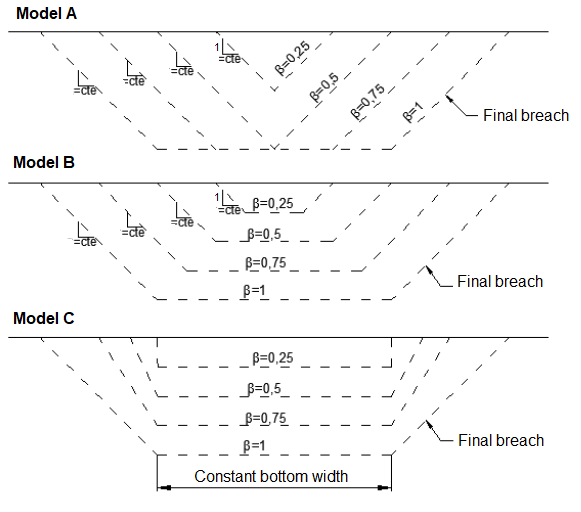
\includegraphics[width=\textwidth]{./graphics/bennani2016}
\caption{Schematic representations of three empirical breach formation models
(adapted from Bennani \cite{Bennani2016})}
\label{fig:froehlich}
\end{figure}
Froehlich \cite{Froehlich2008} used the concept expressed by Brunner
\cite{Brunner2002} who proposed a sine-curve time progression (instead of the
common linear time evolution), reflecting slower growth at the start;
then acceleration and again slow finish of breach development.
In \telemac{2D}, Models A and B are combined and adapted for two-dimensional
simulations as follows:
\begin{itemize}
\item the instantaneous top width of the breach is computed as:
\begin{equation}
\begin{array}{lll}
B(t)=\beta(t)B_f & \text{for}~t\leq T_f &\text{with}~\beta(t)=\dfrac{1}{2}
\left\{1+\sin\left[\pi\left(\dfrac{t}{T_f}-\dfrac{1}{2}\right)\right]\right\}
\end{array}
\end{equation}
\item the instantaneous elevation of the breach bottom is calculated as follows:
\begin{equation}
\begin{array}{lll}
Z_b(t)=Z_{b0}-\beta_1(t)(Z_{b0}-Z_{b,min}) & \text{for}~t\leq T_d &
\text{with}~\beta_1(t)=\dfrac{1}{2}\left\{1+\sin\left[\pi\left(\dfrac{t}{T_d}
-\dfrac{1}{2}\right)\right]\right\}
\end{array}
\end{equation}
\end{itemize}
with $t$ = time in hours (after the initiation of breaching), $B_f$ = final top
width of the breach in meters. Note that $T_f$ and $B_f$ are user-defined.\\
This law can be selected filling the \telkey{BREACHES DATA FILE} with
\begin{lstlisting}[language=bash]
# Option for lateral growth
10
\end{lstlisting}
\subsection{Breaches data file}
In order to give all information about the breach process, the user has to
complete the \telkey{BREACHES DATA FILE}.
When the initial widths of breaches are known, the keyword
\telkey{INITIAL WIDTHS OF BREACHES} must be set to TRUE in the steering file
(default value = NO). Note that in release 8.3 this keyword was in fact
\telkey{INITIAL LENGTHS OF BREACHES} (lengths was later replaced by widths).
If the initial widths are unknown, \telemac{2D} will automatically compute the
initial width for the breaching process. First, the initial width is estimated
as a tenth of the final breach width;
then it is computed as the maximum value between the estimated initial width
and the distance between the central points of the polyline defining the
breach. Indeed in \telemac{2D} we assume that the breaching process will start
at the middle of the polyline.
The breaching zone is thus defined by a polyline of several points associated
to a bandwidth.
The final situation is characterized by a bottom altitude that will be reached
by all the points located in the breaching zone.
%If after the dyke breaching, the bottom level is not constant, it is thus
%necessary to divide the dyke into several breaching polylines.

To avoid errors, the \telkey{BREACHES DATA FILE} has to be written in the
following way (the order of parameters cannot be changed):
\begin{itemize}
\item Number of breaches,
\item Width of the polygon defining the breaches (in m),
\item Option for the breaching initiation (from 1 to 5),
\item If the option of breaching initiation is at a given time (option 1):
breach opening moment in seconds,
\item Duration of the breaching process (in s),
\item Option for lateral growth (from 1 to 10),
\item Final bottom altitude of the breach (in m),
\item If option of breaching initiation corresponds to controlling level of
breach with global node (option 3 and 5): number of global node controlling the breach,
\item If option of breaching initiation is number 4: 3 mesh points have to be given.
One to control the water depth, one to compute the hydraulic head on the channel and
one to compute the hydraulic head on the floodplain,
\item If option of breaching is number 4 or 5: threshold value for difference of hydraulic
head (in m),
\item If option of breaching initiation is not at given time: control level of
the breach (in m),
\item If the user defined formula with two growth rates is used for lateral
growth (option 3): duration for first step, growth rate for step 1 and growth
rate for step 2 (in m/hours),
\item If the Verheij 2003 formula is used for lateral growth (option 9):
critical flow velocity for the initiation of erosion of dyke material (m/s);
$f_1$ and $f_2$ empirical coefficients (/),
\item If the Froehlich formula is used for lateral growth (option = 10):
difference between initial and final elevation of the dyke (m),
\item If the initial width is known: value of initial width (m),
\item Number of points of the polyline defining the breach,
\item Description of the polyline (points with x and y coordinates).
\end{itemize}

%However, the \telkey{BREACHES DATA FILE} is modified as follows:
%
%\begin{itemize}
%\item addition of two new lines for selecting breach opening option.
%These two lines -- comment line and the value for the option -- come after
%the breach duration. The options are selected using:
%\begin{itemize}
%\item 1: for dyke opening by bottom lowering (the old implementation),
%
%\item 2: for dyke opening by widening,
%
%\end{itemize}
%\item the width of polygon defining breach is given for each breach.
%\end{itemize}

A commented example of \telkey{BREACHES DATA FILE} is provided below.
This example is taken from the test case telemac2d/breach.

\begin{lstlisting}[language=bash]
# Number of breaches
3
# Definition of upstream breach
# Width of the polygon defining the breaches
50.0
# Option for the breaching initiation
2
# Duration of the breaching process (0.0 = instantaneous)
300.0
# Option for lateral growth Verheij 2002 (non cohesive)
7
# Final bottom altitude of the breach
5.9
# Control level of the breach
7.2
# Number of points of the polyline
4
# Description of the polyline
2000.0 37.5
2041.0 37.5
2082.0 37.5
2100.0 37.5
# Central breach definition
# Definition of central breach
# Width of the polygon defining the breaches
60.0
# Option for the breaching initiation
3
# Duration of the breaching process (0.0 = instantaneous)
900.0
# Option for lateral growth
10
# Final bottom altitude of the breach
5.5
# Number of global node controlling the breach
9406
# Control level of the breach
6.0
# Difference between initial and final elevation of the dyke
2.049
# Number of points of the polyline
4
# Description of the polyline
2450.0 37.5
2500.0 37.5
2520.0 37.5
2550.0 37.5
# Downstream breach definition
# Width of Polygon defining the breach
10.0
# Option for the breaching process
1
# Start time of the breaching process
2000.0
# Duration of the breaching process (0.0 = instantaneous)
600.0
# Option of lateral growth
# (1= bottom lowering, 2= opening by widening)
1
# Final bottom altitude of the breach
5.0
# Number of points on the dyke axis where the breach will appear
4
# Description of the polyline
2900.0 37.5
2920.0 37.5
2950.0 37.5
3000.0 37.5
\end{lstlisting}

It is worth noting that the duration of the breaching process ($T_f$) is
effectively used in \telemac{2D} to compute the width of the breach in case of
linear laws and the Froehlich law.
For other laws, the breach will continue widening until the final width
(defined by the polyline) will be reached. \\
Despite that, the duration of the breaching process is always considered to
compute the duration of breach deepening ($T_d$).
